\subsection{Comparison of results}
\subsubsection{Quality of deblurring}
\begin{frame}[allowframebreaks]{Comparison of results - Sensitivity to noise}

\begin{figure}
\centering
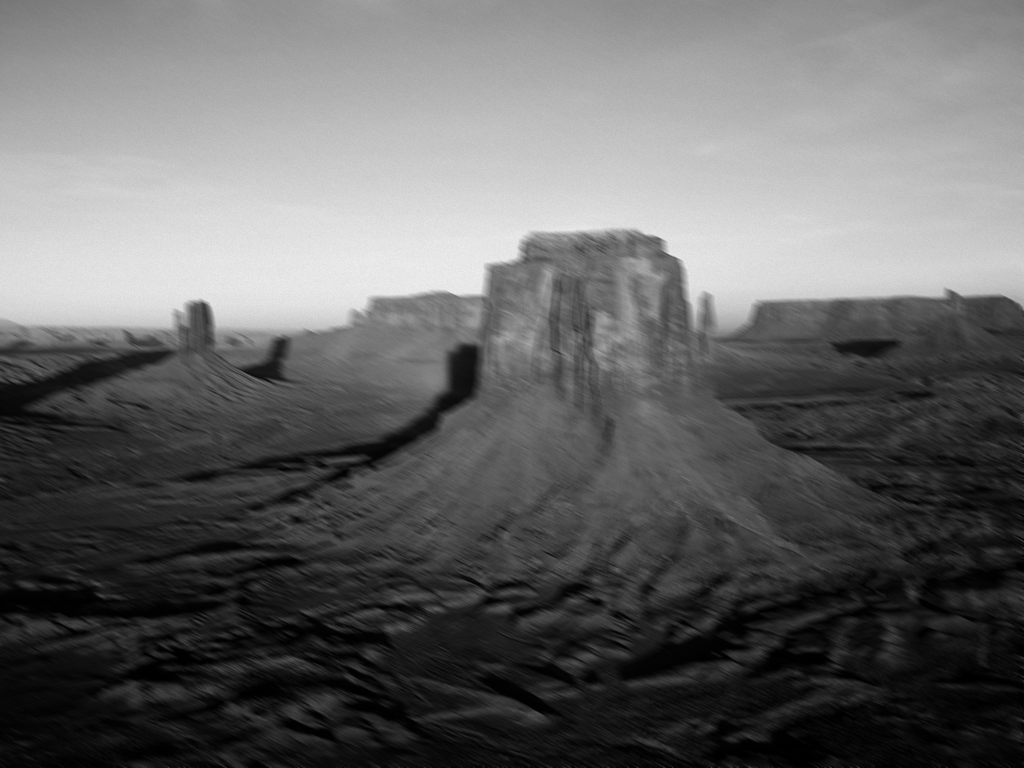
\includegraphics[{scale=0.1}]{../Images/Results/desert/Speckle/input.png}
\caption{Original image whith Speckle noise}
\end{figure}


\begin{figure}
\centering
\begin{subfigure}{0.3\textwidth}
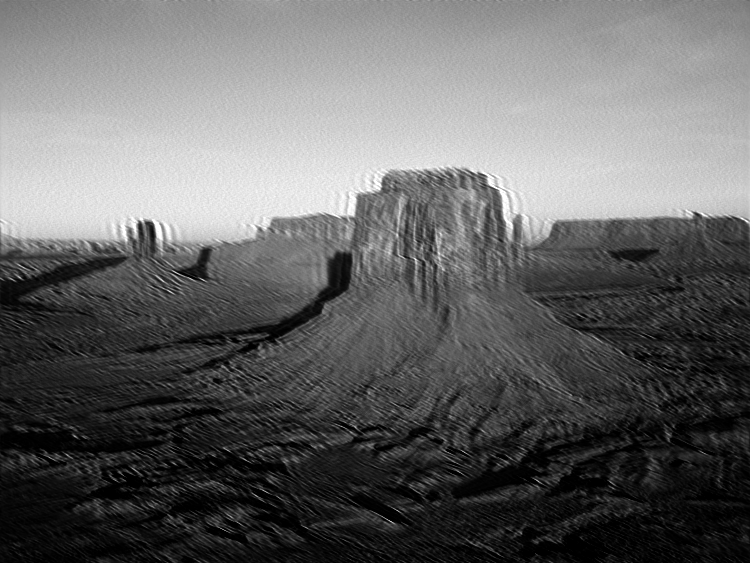
\includegraphics[{width= \textwidth}]{../Images/Results/desert/Speckle/L.png}
\caption{Lucy}
\label{fig:SpeckleL}
\end{subfigure}
~
\begin{subfigure}{0.3\textwidth}
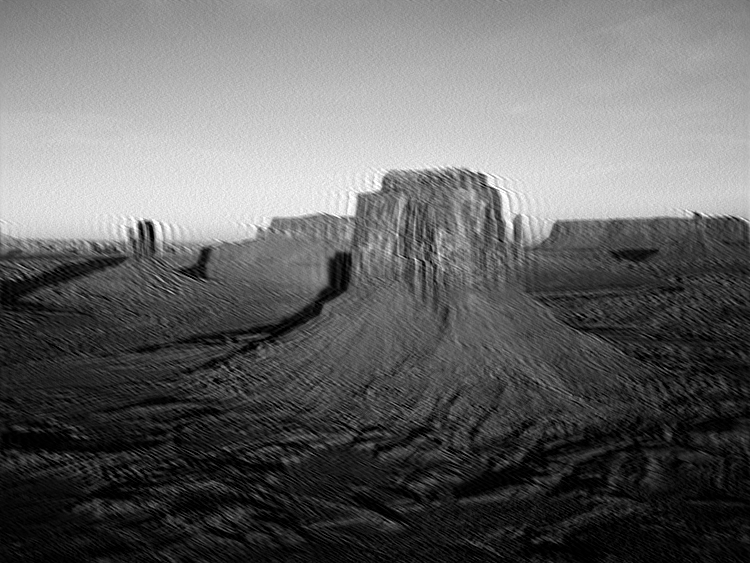
\includegraphics[{width= \textwidth}]{../Images/Results/desert/Speckle/W.png}
\caption{Wiener}
\label{fig:SpeckleW}
\end{subfigure}
~
\begin{subfigure}{0.3\textwidth}
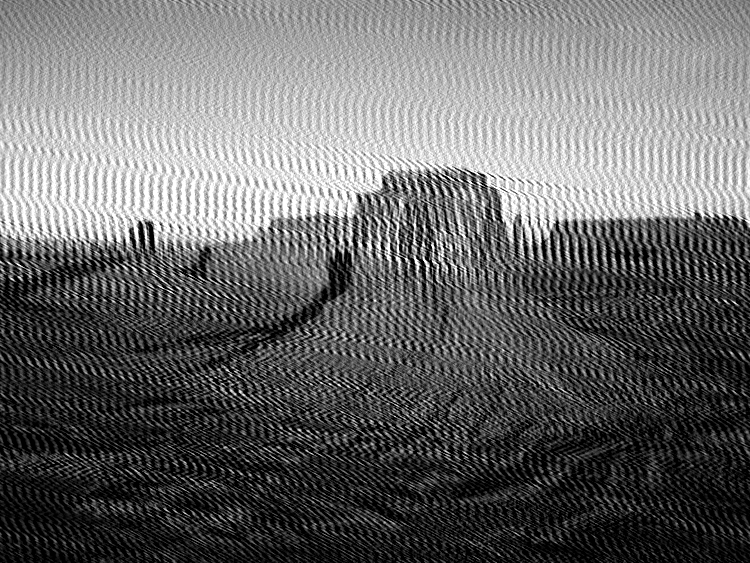
\includegraphics[{width= \textwidth}]{../Images/Results/desert/Speckle/R.png}
\caption{Reguralization}
\label{fig:SpeckleR}
\end{subfigure}
\caption{Image with speckel noise deblurred.}
\end{figure}

\end{frame}


\begin{frame}[allowframebreaks]{Comparison of results - Sensitivity to approximate angle}

\begin{figure}
\centering
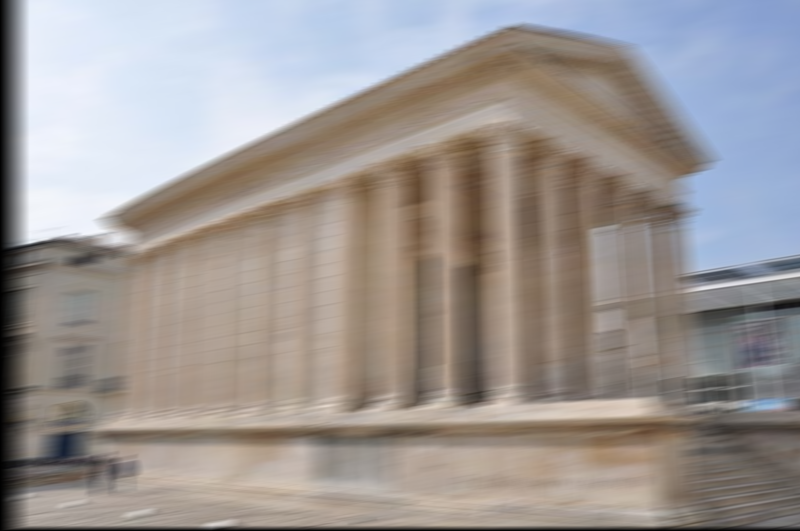
\includegraphics[scale = 0.2]{../Images/Results/NimeAngle/Blurlength30angle10.png}
\caption{Artificial blur: $30$ pixels and $10$ degrees}
\label{fig:nimeOriginal}
\end{figure}

\begin{figure}
\centering
\begin{subfigure}{0.3\textwidth}
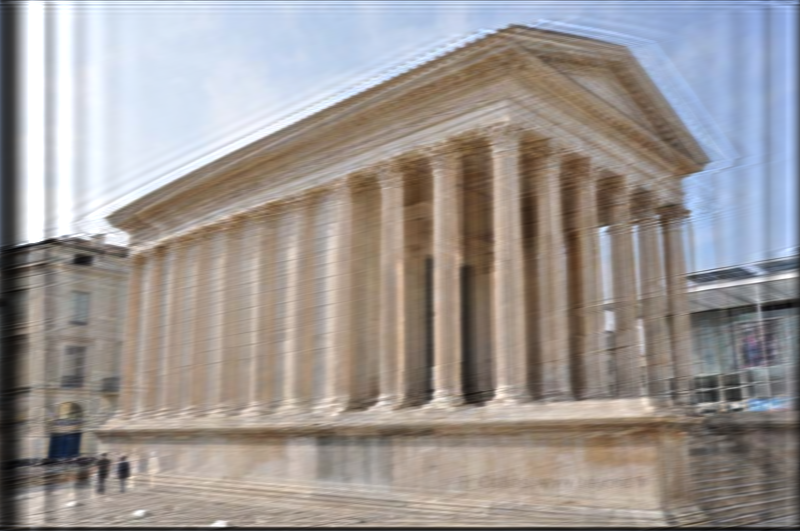
\includegraphics[width= \textwidth]{../Images/Results/NimeAngle/LucyAngle8.png}
\caption{Lucy}
\label{fig:L8}
\end{subfigure}
~
\begin{subfigure}{0.3\textwidth}
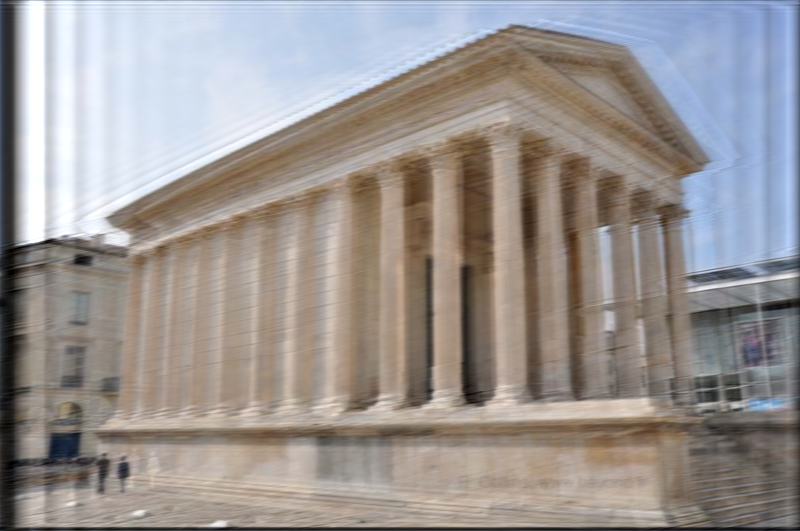
\includegraphics[{width= \textwidth}]{../Images/Results/NimeAngle/WienerAngle8.png}
\caption{Wiener}
\label{fig:W8}
\end{subfigure}
~
\begin{subfigure}{0.3\textwidth}
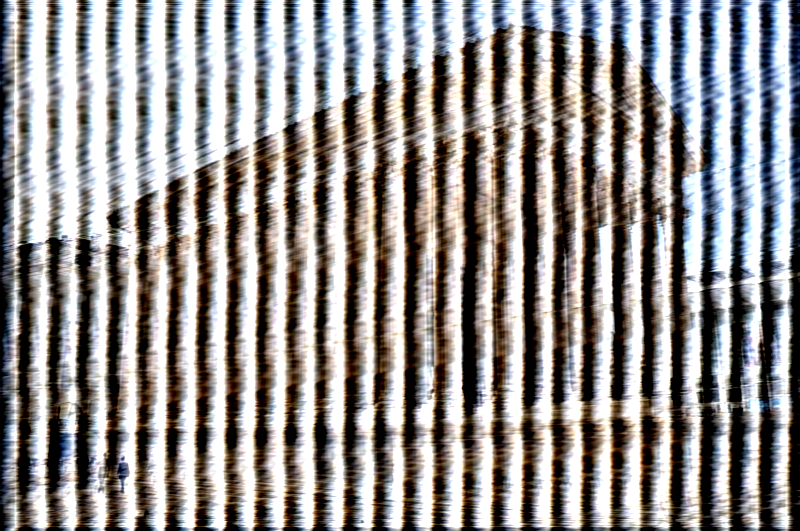
\includegraphics[{width= \textwidth}]{../Images/Results/NimeAngle/RegAngle8.png}
\caption{Reguralization}
\label{fig:R8}
\end{subfigure}
\caption{Image deblurred with an angle of 8 degrees and the right length.}
\end{figure}

\end{frame}


\begin{frame}[allowframebreaks]{Comparison of results - Sensitivity to approximate length}

\begin{figure}
\centering
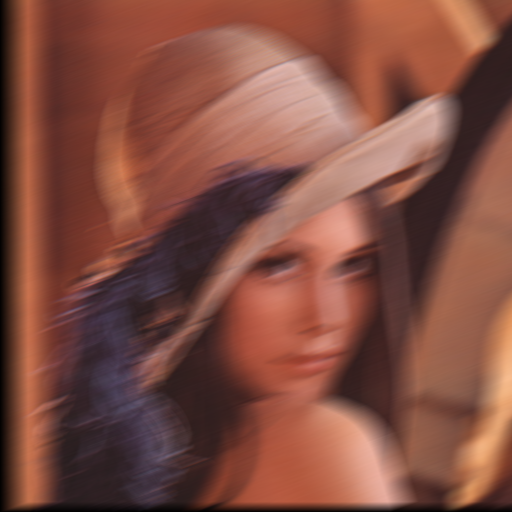
\includegraphics[{scale=0.2}]{../Images/Results/Lena/Blur20deg30length/ArtificialBlurred.png}
\caption{Artificial blur: $30$ pixels and $0$ degrees}
\end{figure}

\begin{figure}
\centering
\begin{subfigure}{0.3\textwidth}
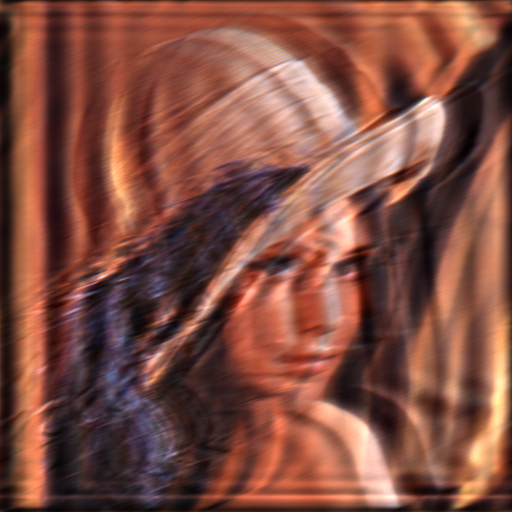
\includegraphics[{width= \textwidth}]{../Images/Results/Lena/Blur20deg30length/L40.png}
\caption{Lucy}
\label{fig:L40}
\end{subfigure}
~
\begin{subfigure}{0.3\textwidth}
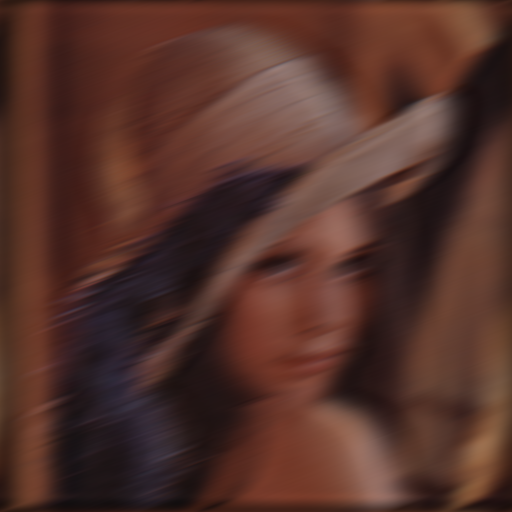
\includegraphics[{width= \textwidth}]{../Images/Results/Lena/Blur20deg30length/W40.png}
\caption{Wiener}
\label{fig:W40}
\end{subfigure}
~
\begin{subfigure}{0.3\textwidth}

\includegraphics[{width= \textwidth}]{../Images/Results/Lena/Blur20deg30length/R40.png}
\caption{Reguralization}
\label{fig:R40}
\end{subfigure}
\caption{Image deblurred with length estimation = $40$ pixels and correct angle.}
\end{figure}

\end{frame}

\subsubsection{Computation time}
\begin{frame}{Comparison of results - Computation time}
\begin{figure}[h!]
\centering
\begin{subfigure}{0.4\textwidth}
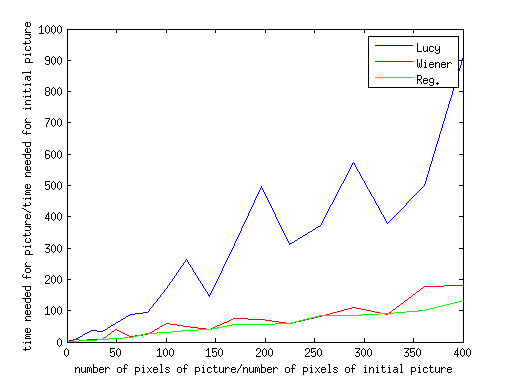
\includegraphics[{width= \textwidth}]{../Images/ComplexityRel.png}
%\caption{time needed to compute `` the picture/ the smallest picture'' - y-axis and number of pixels of the `` picture / smallest picture'' - x-axis.}
\end{subfigure}~
\begin{subfigure}{0.4\textwidth}
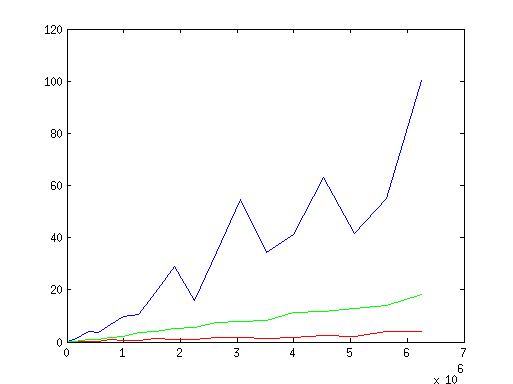
\includegraphics[{width= \textwidth}]{../Images/ComplexityAbs.png}
%\caption{Time  needed to compute the picture on the y-axis, number of pixels of the picture on the x-axis.}
\end{subfigure}
\caption{Complexity of our different algorithms. The blue line is for \texttt{deconvLucy} (16 iterations), the red one for \texttt{deconvwnr} and the green one for \texttt{deconvreg}.}
\label{fig:Complexity}
\end{figure}

\end{frame}
\subsubsection{Conclusion}
\begin{frame}{Comparison of results - Conclusion}
\begin{itemize}
\item Lucy : the most robust but the slowest when the number of pixels rises 
\begin{itemize}
\item if low number of pixels or some time available;
\end{itemize}
\item Wiener : the fastest but some times poor results 
\begin{itemize}
\item Good compromise;
\end{itemize} 
\item Regularisation : the most sensitive to errors 
\begin{itemize}
\item sould be avoided, slower and worse than Wiener.
\end{itemize}
\end{itemize}

\end{frame}
